\documentclass[11pt]{article}
\usepackage[T1]{fontenc}
\usepackage{booktabs}
\usepackage{lipsum}
\usepackage{tikz}
\usepackage{amsmath}
\usepackage{amssymb}
\usepackage{graphicx}
\usepackage{enumitem}
\usepackage{float}

\title{LaTeX Demo Document}
\author{}
\date{}

\begin{document}

\maketitle

\section{Introduction}
\lipsum[1][1-3]

\section{Lists}

\subsection{Itemized List}
\begin{itemize}[noitemsep]
\item First item with some text to show wrapping.
\item Second item with inline math: $E=mc^2$ and a display style equation below:
\begin{equation*}
\sum_{i=1}^{n} i = \frac{n(n+1)}{2}
\end{equation*}
\item Third item with a reference to Figure~\ref{fig:simple}. See below.
\end{itemize}

\subsection{Enumerated List}
\begin{enumerate}[noitemsep]
\item First ordered item.\label{itm:first}
\item Second ordered item with a footnote\footnote{This is a footnote.}.
\item Third ordered item referencing item~\ref{itm:first}.
\end{enumerate}

% FIXME: Fix this

\section{Figures and Tables}

\begin{figure}[H]
\centering
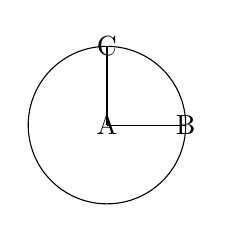
\begin{tikzpicture}
\draw (0,0) circle (1cm);
\draw (0,0) -- (1,0);
\draw (0,0) -- (0,1);
\node at (0,0) {A};
\node at (1,0) {B};
\node at (0,1) {C};
\end{tikzpicture}
\caption{A simple TikZ graph with nodes A, B, and C.}\label{fig:simple}
\end{figure}

\begin{table}[H]
\centering
\begin{tabular}{lcc}
\toprule
\textbf{Metric} & \textbf{Value} & \textbf{Unit} \\
\midrule
\lipsum[2][1] & 42 & m/s \\
\lipsum[3][1] & 3.14159 & kg \\
\bottomrule
\end{tabular}
\caption{A table using booktabs.}\label{tab:metrics}
\end{table}

\section{Math and Symbols}
Inline math: $x^2 + y^2 = z^2$. Display style:

\begin{equation*}
\int_{a}^{b} f(x)\,dx = F(b) - F(a)
\end{equation*}
\begin{figure}[htbp]
  \centering
  \begin{tikzpicture}[scale=1.2]
    % Axes
    \draw[->] (-0.5,0) -- (5.5,0) node[right] {$Q$};
    \draw[->] (0,-0.5) -- (0,5.5) node[above] {$P$};
    % Demand curve (blue)
    \draw[blue, thick] (0,4) -- (4,0) node[midway, below right] {$D$};
    % Supply curve (red)
    \draw[red, thick] (0,2) -- (4,4) node[midway, above right] {$S$};
    % Intersection point
    \coordinate (Pstar) at (1,3);
    \fill (Pstar) circle (2pt) node[above left] {$P^{*}$,$Q^{*}$};
  \end{tikzpicture}
  \caption{Supply and demand curves.}
  \label{fig:supply-demand}
\end{figure}

\section{Conclusion}
\lipsum[4][1-3]



\end{document}